\documentclass{article}

\usepackage[margin=1in]{geometry}
\usepackage{fancyhdr}
\usepackage{amssymb}
\usepackage[most]{tcolorbox}
\usepackage{listings}
\usepackage{siunitx}
\usepackage{cite}
\usepackage{wrapfig}
\usepackage{hyperref}

\title{The Search for Multiquark States at the Large Hadron Colldier}
\author{Simon Lavoie}

\begin{document}

\newpage
\maketitle

\begin{abstract}
  Baryonic matter, of which we are primarily made of, is itself composed of three quarks.
  These baryons include the proton and neutron, which we know as the core constituents of the 
  nucleus. There also exists the traditional mesons, which are composed of only two quarks. This begs the question:
  do particles composed of groups larger than a trio of quarks exist? The short answer is yes, 
  with the first observation of a tetraquark - a particle composed of four quarks - being made 
  in 2003 by the Belle Collaboration \cite{MultiquarkDiscovery}.
  In this paper, the search for possible multiquark states using strange particles, namely, the 
  $K^0_s$ meson and the $\Lambda^0$ baryon is done using data collected by the ATLAS detector 
  of proton-proton collisions at a center-of-mass energy of $\sqrt{s} =$ \SI{13.6}{TeV}. Minimum
  bias data from 2015 having an integrated luminosity of \SI{21.559}{nb}$^{-1}$ is used. Secondary 
  vertices are marked as either a $K^0_s$ or $\Lambda^0$ using strict cuts and their invariant mass and 
  lifetimes are fitted for verification. A low energy resonant state of the $K^0_sK^0_s$ invariant 
  mass distribution was detected at 1524.40 $\pm$ 4.83 MeV which likely corresponds to the 
  $f_2'(1525)$ state. With this known signal identified, a bump hunt is performed on the higher-energy
  range of the $K^0_sK^0_s$, $K^0_s\Lambda^0$ and $\Lambda^0\Lambda^0$ invariant mass spectra
  in search for possible tetraquark, pentaquark and hexaquark states. The results of this bump hunt 
  were inconclusive, with no signal exceeding a significance of $3\sigma$. Further analysis is required
  to determine the presence of higher energy resonances. 

\end{abstract}





\newtcblisting{mycode}{%
    boxrule=0.5pt,
    colback=white,
    listing only,
    listing options={basicstyle=\ttfamily, numbers=left},
}
\lstset{basicstyle=\ttfamily}
\pagestyle{fancy}
\lhead{Simon Lavoie}
\chead{}
\rhead{Summer Research Period: May 1st - August 20 2024}
\lfoot{}
\cfoot{}
\rfoot{}
\renewcommand{\headrulewidth}{1pt}

\today






\section{Introduction}
From the discovery of various exotic particles such as pions in the 50's to that of the Higgs
boson in 2012, the advent of particle accelerators brought about new discoveries in particle physics,
bolstering our grasp on the standard model - a guage theory which describes three out of the four
fundamental forces, that being the weak, strong, and electromagnetic forces \cite{KLDiscovery}, \cite{HiggsDiscovery}. 
As the collision energies of particle accelerators steadily increase, new discoveries of higher mass particles 
can be made. 
Multiquarks are an example of these higher mass particles, being made up of collections of quarks
whose number exceeds that of the usual two or three we observe in mesons and baryons respectively.
Such particles are not forbidden by the standard model, and a proper identification of multiquark 
states may help in our understanding of quantum chromodynamics (QCD) - a core component of the standard 
model which describes the interactions between quarks and the elementary particle which mediates 
the strong interaction between them: the gluon. Thus, this work searches for multiquark states 
through the possible decay products of tetraquarks, pentaquarks and hexaquarks. The decay channels
are as follows:

\begin{align*}
\text{Tetraquark}: A &\rightarrow K^0_sK^0_s \\
\text{Pentaquark}: B &\rightarrow K^0_s\Lambda^0 \\
\text{Hexaquark}:  C &\rightarrow \Lambda^0\Lambda^0
\end{align*}

Where the $K^0_s$ meson is a neutral kaon composed of a down quark $(d)$ and an
anti-strange quark $(\bar{s})$, and the $\Lambda^0$, known as the Lambda baryon,
is composed of an up, down and strange quark $(uds)$. Quarks are known to
possess one of the three fundamental color charges, of which there are three:
Red, Green and Blue. According to the color confinement principle, a core tenet
of QCD, color-charged particles such as quarks cannot be isolated, and thus
quarks combine to form color-neutral hadrons called singlet states. Nothing
forbids the creation of a singlet state composed of two quarks and two
antiquarks $(qq\bar{q}\bar{q})$, a particle called a tetraquark which would be
categorized as an exotic meson since, despite not being composed of a single
quark-antiquark pair, it nonetheless possesses a meson's characteristic trait of
being a hadron with a baryon number of zero. Similarly, nothing forbids the
combination of a color-neutral baryon and a quark-antiquark pair $(qqqq\bar{q})$
which we would call a pentaquark. A combination of two baryons or three
quark-antiquark pairs could also exist $(q^6 \text{ or } q^3\bar{q}^{3})$, which
are both example of hexaquarks.

\subsection{Event Reconstruction}
The $K^0_s$ and $\Lambda^0$ are chosen as objects of study due to their decay
products being easily identifiable within the ATLAS (A Torroidal LHC Apparatus) 
detector. The $K^0_s$ is
known to decay into two charged pions $(\pi^+\pi^-)$ with a branching ratio of
$69.20 \pm 0.05 \unit{\%}$ \cite{KBranchingRatio} and the $\Lambda^0$ decays
into into a proton and a pion $(p^+\pi^-)$ with a branching ratio of $63.9 \pm
0.5 \unit{\%}$ \cite{LBranchingRatio}. These charged particles are traced back to 
a secondary vertex (denoted $V0$) and the $K^0_s$ or $\Lambda^0$ invariant mass is reconstructed using the
respective decay product's energies and momenta.
The invariant mass of this two-particle 
decay (in nautral units) is given by:
\begin{equation}
M = \sqrt{(E_1 + E_2)^2 - ||p_1 + p_2||^2}.\label{equation: invmass} 
\end{equation}
Once two secondary vertices are reconstructed within a single event, the process 
can be repeated to reconstruct the invariant mass of the primary vertex, which is the point 
of the $p-p$ collision, once again using 
equation \ref{equation: invmass}. The resulting primary vertex invariant mass distribution can then be 
searched for possible multiquark resonances.
Before this can be done, however, cuts must be placed on the reconstructed $V0$s
to reduce the background and ensure no misidentification of particles occur.
\begin{figure}[!h]
\includegraphics*[width=0.9\textwidth]{Figs/AllThree.png} 
\caption{Tetraquark, pentaquark and hexaquark decay chains, respectively.}
\end{figure}

\section{Methods}
Each $V0$ is considered a potential $K^0_s$ and $\Lambda^0$ candidate and is subject 
to a series of cuts in order to properly categorize the secondary vertex. This is because 
the ATLAS detector obtains only data on the momentum and charge of the pions and protons.
The trouble lies in differentiating the $p^+$ from $\pi^+$, as the  $\pi^-$ are easily 
identifiable. In order to accomplish this, the invariant mass of each secondary vertex 
is computed twice: once with the proton mass, and another with the pion mass. The cuts are 
then used to determine which hypothesis was correct, as well as reduce the overall background.
The cuts are as follows:\\
\vspace{-24pt}
\begin{wrapfigure}[13]{l}{0.40\textwidth}
  \includegraphics[width=0.39\textwidth]{Figs/KinematicVariables.png}
  \caption{\small Kinematic variables of a $K^0_s \rightarrow \pi^+\pi^-$ decay process.}\label{figure: KinematicVariables}
\end{wrapfigure}

\begin{itemize}
    \item Cut on pointing angle: $\cos(\theta)$ 
    \item Cut on transverse momentum: $p_T$
    \item Cut on distance travelled: $d$
    \item Cut on invariant mass: $m_{\pi^+\pi^-}$
    \item Cut on invariant mass: $m_{p^+\pi^-}$
\end{itemize}

With $p_T$ and $\cos(\theta)$ being given by:
\begin{equation}
    p_T = \sqrt{p_x^2 + p_y^2}
\end{equation}
\begin{equation}
    \cos(\theta) = \frac{\Delta x p_x + \Delta y p_y}{p_Td}
\end{equation}
Where $\Delta x$ and $\Delta y$ are the differences in $x$ and $y$ coordinates between the primary 
and secondary vertices and the equation for $\cos(\theta)$ comes from the dot product between the 
vectors $\vec{R}$ (the path vector whose magnitude is $d$) and $\vec{p}$, the reconstructed momentum, 
as per figure \ref{figure: KinematicVariables}.


\subsection{Cut on Pointing Angle}
The most impactful cut which can be placed on a secondary vertex is the cut on the pointing angle. 
This cut removes a significant amount of the background as it is incredibly effective at ensuring the 
charged decay products originate from the same vertex. The result of requiring the cosine of the 
pointing angle to exceed 0.9998 can be seen in figures \ref{figure: KMassCosCut} and \ref{figure: LMassCosCut}
for the kaon and lambda respectively.
\begin{figure}[!h]
\centering
\begin{minipage}{.48\textwidth}
\centering
\includegraphics[width=\textwidth]{Figs/KMassCosCut.png}
\caption{\small $K_s^0$ invariant mass histogram before and after cut on pointing angle.}
\label{figure: KMassCosCut}
\end{minipage}%
\hfill
\begin{minipage}{.48\textwidth}
\centering
\includegraphics[width=\textwidth]{Figs/LMassCosCut.png}
\caption{\small $\Lambda^0$ invariant mass histogram before and after cut on
pointing angle.} \label{figure: LMassCosCut}
\end{minipage}
\end{figure}

\subsection{Cut on Transverse Momentum}
The next cuts applied are those on the transeverse momentum. Plotting $p_T$
versus the $K_s^0$ and $\Lambda^0$ invariant mass distributions reveal clear
signals around a mass of \SI{497}{MeV} and \SI{1115}{MeV} corresponding to their
PDG mass values respectively. Figure \ref{figure: LpTCut} reveals a significant
background below a transverse momentum of \SI{500}{MeV}, whereas figure
\ref{figure: KpTCut} shows the transverse momentum to be fairly localized near
the kaon mass.
\begin{figure}[!h]
\centering
\begin{minipage}{.48\textwidth}
\centering
\includegraphics[width=\textwidth]{Figs/Kaon_pT_vs_InvMass.png}
\caption{\small $p_T$ versus $K_s^0$ invariant mass histogram with a cut for $p_T$ values below \SI{400}{MeV}.}
\label{figure: KpTCut}
\end{minipage}%
\hfill
\begin{minipage}{.48\textwidth}
\centering
\includegraphics[width=\textwidth]{Figs/Lambda_pT_vs_InvMass.png}
\caption{\small $p_T$ versus $\Lambda^0$ invariant mass histogram with a cut for $p_T$ values below \SI{500}{MeV}.}
\label{figure: LpTCut}
\end{minipage}
\end{figure}

\subsection{Cut on Distance Travelled}
A cut on the distance travelled between the primary and secondary vertices is
then placed on the data. This cut is effective at reducing background by
removing particles whose lifetime is shorter than that of the $K_s^0$ or
$\Lambda^0$ as the lifetime of a particle is related to its distance by 

\begin{equation}
    \label{equation: distance}
    d = \beta\gamma c\tau,
\end{equation}

where $d$ is the average decay length, $\beta$ is the ratio between the particle's velocity and the speed of light, 
$\gamma = 1/\sqrt{1-\beta^2}$ is the Lorentz factor, and $\tau$ is the mean lifetime. Rearranging equation \ref{equation: distance}
and writing $\gamma$ in terms of the momentum using $p = \gamma mv$ we obtain:

\begin{equation}
    \label{equation: time}
    \tau = \frac{dm}{p}
\end{equation}

Thus, as can be seen in figures \ref{figure: KDistance} and \ref{figure:
LDistance}, cuts were placed enforcing a minimum distance - and therefore
lifetime on the secondary vertices to further reduce background.

\begin{figure}[!h]
\centering
\begin{minipage}{.48\textwidth}
\centering
\includegraphics[width=\textwidth]{Figs/Kaon_d_vs_InvMass.png}
\caption{\small $d$ versus $K_s^0$ invariant mass histogram with a cut for distances below \SI{4}{mm}.}
\label{figure: KDistance}
\end{minipage}%
\hfill
\begin{minipage}{.48\textwidth}
\centering
\includegraphics[width=\textwidth]{Figs/Lambda_d_vs_InvMass.png}
\caption{\small $d$ versus $\Lambda^0$ invariant mass histogram with a cut for distances below \SI{17}{mm}.}
\label{figure: LDistance}
\end{minipage}
\end{figure}

A lifetime analysis is later performed, outlined in section \ref{section:
lifetime}, allowing for the placement of a cut on the maximum distance travelled 
by the secondary vertices.

\subsection{Cut on $K_s^0$ and $\Lambda^0$ Mass}

\begin{wrapfigure}[20]{l}{0.60\textwidth}
  \includegraphics[width=0.59\textwidth]{Figs/LMassVsKMass.png}
  \caption{\small $\Lambda^0$ vs. $K_s^0$ invariant mass distributions with cuts
  to avoid misidentification of particles. $K_s^0$ candidates having a
  $\Lambda^0$ mass less than \SI{1125}{MeV} and $\Lambda^0$ candidates having a
  $K_s^0$ mass greater than \SI{475}{MeV} are rejected.}
  \label{figure: LMassVsKMass}
\end{wrapfigure}

Another cut which can be placed is around the mass signal itself. 
This cut is likely the most obvious one to place, as the mass of the $K_s^0$ and
$\Lambda^0$ are well known and a significant portion of the background seen in
the plots of the previous sections can be removed by simply cutting around the
mass signal.  This is not without some difficulty, however, as certain secondary
vertices happen to pass both the series of $K_s^0$ and $\Lambda^0$ cuts,
including that of the mass signal cut. As can be seen on figure 
\ref{figure: LMassVsKMass}, there are secondary vertices whose reconstructed 
kaon mass $m_{\pi^+\pi^-}$ lies within the vertical streak near \SI{497}{MeV},
but whose Lambda mass $m_{p^+\pi^-}$ simultaneously lies within the horizontal 
streak near \SI{1115}{MeV}. These secondary vertices can be mistaken as being both
kaons and Lambdas and are therefore rejected from this analysis due to their 
ambiguity.

\subsection{Cut on $K_s^0$ and $\Lambda^0$ Lifetime}\label{section: lifetime}
The lifetime distribution of all secondary vertices passing the previous cuts, as given by equation \ref{equation: time} can be 
fitted to a signal plus background model of the form:
\begin{equation}
    \label{equation: lifetime_fit_model}
    y(t) = C_0 + C_be^{-t/\tau_b} + C_se^{-t/\tau_s}
\end{equation}
Where $C_0$ and $C_b$ are constants modelling the background having a lifetime of $\tau_b$, while $C_s$ and $\tau_s$
are the constant and lifetime of the signal respectively.

\begin{figure}[!h]
\centering
\begin{minipage}{.48\textwidth}
\centering
\includegraphics[width=\textwidth]{Figs/KaonLifetime.png}
\caption{\small $K_s^0$ lifetime distribution with a fitted mean lifetime of 
         $78.9 \pm 0.1$ \unit{ps} compared to a PDG mean lifetime of $89.56 \pm 0.03$ \unit{ps}\cite{KBranchingRatio}.}
\label{figure: KDistance}
\end{minipage}%
\hfill
\begin{minipage}{.48\textwidth}
\centering
\includegraphics[width=\textwidth]{Figs/LambdaLifetime.png}
\caption{\small $\Lambda^0$ lifetime distribution with a fitted mean lifetime of 
         $24.7 \pm 20$ \unit{ns} compared to a PDG mean lifetime of $26.32 \pm 0.02$ \unit{ns}\cite{LBranchingRatio}.}
\label{figure: LDistance}
\end{minipage}
\end{figure}

The point at which the signal contribution of the overall fit drops close to zero 
designates the ideal region to place a cut on the maximum lifetime of a secondary vertex,
as it ensures maximal background reduction while minimizing signal reduction. This 
maximum lifetime is completely analogous to setting a maxiumum distance travelled.
Furthermore, fitting this data according to equation \ref{equation: lifetime_fit_model}
yields the particle's mean lifetime which can be compared to reference values to 
ascertain the reliability of this cut.

\subsection{Summary and Effect of All Cuts}\label{section: All Cuts}

\begin{figure}[!h]
\centering
\begin{minipage}{.48\textwidth}
\centering
\includegraphics[width=\textwidth]{Figs/KMass.png}
\caption{\small $K_s^0$ invariant mass histogram with all cuts progressively
displayed. The distribution is fitted with a Breit-Wigner function for the
signal and a quadratic function for the background. The signal is centered at
$497.85 \pm 0.01$ \unit{MeV} compared to the $K_s^0$ PDG mass of $497.61 \pm
0.01$ \unit{MeV}\cite{KBranchingRatio}.}
\label{figure: KMass}
\end{minipage}%
\hfill
\begin{minipage}{.48\textwidth}
\centering
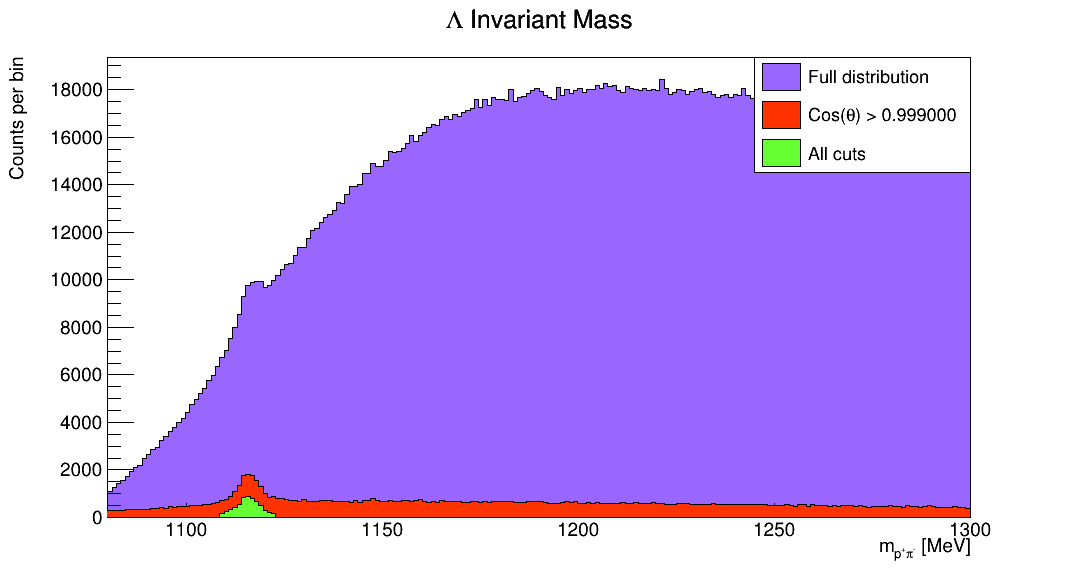
\includegraphics[width=\textwidth]{Figs/LMass.png}
\caption{\small $\Lambda^0$ invariant mass histogram with all cuts progressively
displayed. The distribution is fitted with a Breit-Wigner function for the
signal and a quadratic function for the background. The signal is centered at
$1115.95 \pm 0.01$ \unit{MeV} compared to the $\Lambda^0$ PDG mass of $1115.683 \pm
0.006$ \unit{MeV}\cite{LBranchingRatio}.}
\label{figure: KMass}
\end{minipage}
\end{figure}


With all these cuts put in place, the background is significantly reduced 
allowing for the reconstruction of multiquarks. Events are selected by requiring 
exactly two kaons, two Lambdas or one of each. The two secondary 
vertices are then used to compute the invariant mass of the multiquark, and the resulting 
distributions are plotted. 

\begin{table}[h!]
\caption{Cuts Placed on Secondary Vertices}
\label{tab:my-table}
\centering
\begin{tabular}{lcccc}
\hline
\textbf{Variable}                    & \multicolumn{1}{l}{\textbf{$K_s^0$-min}} & \multicolumn{1}{l}{\textbf{$K_s^0$-max}} & \multicolumn{1}{l}{\textbf{$\Lambda^0$-min}} & \multicolumn{1}{l}{\textbf{$\Lambda^0$-max}} \\ \hline
Pointing Angle - $\cos(\theta)$                       & 0.9998                                                    & N/A                                                       & 0.9998                                                        & N/A                                                           \\
Transverse Momentum - $p_T$ [MeV]                 & 400                                                       & N/A                                                       & 500                                                           & N/A                                                           \\
Distance - $d$ [mm]                               & 4                                                         & N/A                                                       & 17                                                            & N/A                                                           \\
$K_s^0$ Invariant Mass - $m_{\pi^+\pi^-}$ [MeV]   & 480                                                       & 520                                                       & 1125                                                          & N/A                                                           \\
$\Lambda^0$ Invariant Mass - $m_{p^+\pi^-}$ [MeV] & N/A                                                       & 475                                                       & 1105                                                          & 1125                                                          \\ 
Lifetime - $\tau$ [ns]                            & N/A                                                       & 0.6                                                       & N/A                                                           & 1.2                                                           \\ \hline
\end{tabular}
\end{table}

\section{Results}
\subsection{Tetraquark Invariant Mass Distribution}
\begin{wrapfigure}[14]{r}{0.60\textwidth}
  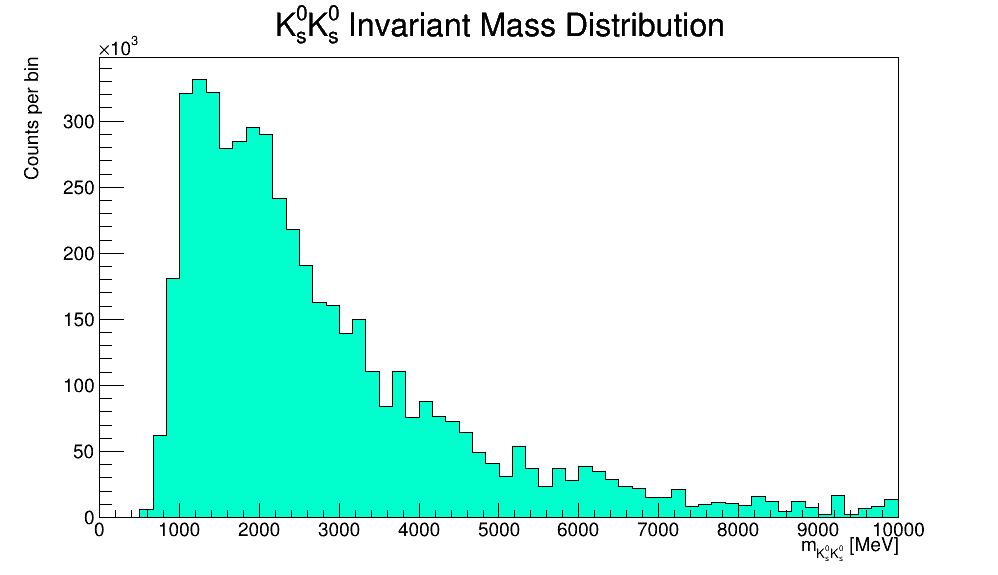
\includegraphics[width=0.59\textwidth]{Figs/KKInvMass.png}
  \caption{\small Tetraquark invariant mass distribution.}\label{figure: KKInvMass}
\end{wrapfigure}

The tetraquark invariant mass distribution is searched for known resonances.
These known resonances exist in the 1100-1800 \unit{MeV} range, and have been
found by the HERA experiment \cite{HERA} and the L3 experiment \cite{L3} among
others. The presence of these resonances in the reconstructed $K_s^0K_s^0$
invariant mass distribution indicates an adequate reduction of the background,
which potentially allows for the discovery of new resonances in the higher
energy range. The $K_s^0K_s^0$ invariant mass distribution is shown in figure
\ref{figure: KKInvMass}.

\vspace{20pt}

\begin{figure}[!h]
\centering
\begin{minipage}{.48\textwidth}
\centering
\includegraphics[width=0.85\textwidth]{Figs/L3KsKs.png}
\caption{\small $K_s^0K_s^0$ invariant mass distribution from the L3 experiment \cite{L3}.}
\label{figure: L3}
\end{minipage}%
\hfill
\begin{minipage}{.48\textwidth}
\centering
\includegraphics[width=0.85\textwidth]{Figs/HERA.png}
\caption{\small $K_s^0K_s^0$ invariant mass distribution from the HERA experiment \cite{HERA}.}
\label{figure: HERA}
\end{minipage}
\end{figure}

\begin{wrapfigure}[18]{l}{0.60\textwidth}
  \includegraphics[width=0.59\textwidth]{Figs/KKInvMassResult.png}
  \caption{\small Tetraquark invariant mass distribution low energy resonance 
            with a signal fitted with a Gaussian distribution having a mean of
            $1524.40 \pm 4.83$ \unit{MeV} and a background fitted with a cubic
            polynomial.}\label{figure: KKInvMassResult}
\end{wrapfigure}

A low energy resonance is detected at 1524.40 $\pm$ 4.83 MeV in the $K^0_sK^0_s$
invariant mass distribution, as can be seen in figure \ref{figure: KKInvMassResult}.
This likely corresponds to the $f_2'(1525)$ state,
a well known resonance which has been observed by the L3 experiment \cite{L3}
and the HERA experiment \cite{HERA} as can be seen in figures \ref{figure: L3}
and \ref{figure: HERA}. This resonance is the largest observed in the previously 
cited papers, and unfortunately the only one observed in this analysis. The search 
for higher energy resonances is ongoing, and efforts are being made to further 
reduce the background in hopes that other known resonances can 
be observed, indicating the possibility of finding new resonances in the higher 
energy ranges. In searching for new resonances in the higher energy range, a 
bump hunt is performed on the $K^0_sK^0_s$, $K^0_s\Lambda^0$ and $\Lambda^0\Lambda^0$ 
distributions. This is done by making multiple copies of the original distribution 
with a single bin missing, and fitting the background with an exponential function of 
polynomial order to the remaining data. The difference between the height of the missing 
bin and the evaluated background at that point is then taken to compute the significance 
of the bin in question. The significance is given by the distance over the error of the bin,
which is simply given by the square root of the bin's value. The results of this bump hunt 
were inconclusive, with no bin having a significance exceeding that of $3\sigma$, which is 
the lower limit for what may be considered a potential discovery in the field of particle 
physics. Further analysis is required to determine the presence of higher energy
resonances. 


\section{Conclusion}
The search for multiquark states using minimum bias data from the ATLAS detector 
of proton-proton collisions at a center-of-mass energy of $\sqrt{s} =$ \SI{13.6}{TeV}
has yielded a low energy resonance in the $K^0_sK^0_s$ invariant mass distribution at 
1524.40 $\pm$ 4.83 MeV, likely corresponding to the $f_2'(1525)$ state. 
This demonstrates an adequate reconstruction of the $K^0_s$ meson and $\Lambda^0$ baryon
and reveals the effectiveness of the cuts placed on the secondary
vertices to reduce background. The search for other known resonances is ongoing,
with a bump hunt performed on the $K^0_sK^0_s$, $K^0_s\Lambda^0$ and $\Lambda^0\Lambda^0$
invariant mass distributions. Further reduction of the background is required to 
ascertain the presence of higher energy resonances.


\section{Acknowledgements}
I would like to thank my supervisor, Prof. François Corriveau, for his guidance and 
support throughout this project. I would also like to thank the ATLAS collaboration 
for providing and treating the data used in this analysis, and the 
current and previous members of the McGill ATLAS group for their support and advice.
This work was a replication of the work done by Antara Paul and Cole Coughlin, 
whose code was adapted to a new software release and used to perform the
analysis presented in this paper.

% Chi squared of lifetime fits are awful. Is it even worth showing lifetime plots if this is the case?
%Should I go into detail about what minimum bias is (requires background on
%luminosity)\\ %Should I go into detail about the coordinate system\\ %How about
%talking about the ATLAS detector in general\\


\bibliographystyle{plain}  
\bibliography{bibliography} 

\end{document}

